\documentclass[a4paper]{article}
\usepackage{algorithmicx}
\usepackage{algpseudocode}
\usepackage{graphicx}
\usepackage{vmargin}
\usepackage[utf8]{inputenc}
\setpapersize{A4}
\setmargins{2.5cm}       % margen izquierdo
{1.5cm}                        % margen superior
{16.5cm}                      % anchura del texto
{23.42cm}                    % altura del texto
{10pt}                           % altura de los encabezados
{1cm}                           % espacio entre el texto y los encabezados
{0pt}                             % altura del pie de página
{2cm}                           % espacio entre el texto y el pie de página

\begin{document}
\section{Caballos salvajes}
\subsection{Problema a resolver}
El problema est\'a dado por encontrar, dado un tablero de $n$ x $n$ posiciones y una cantidad $k$ de caballos (en el contexto del ajedrez) ubicados en dicho tablero, una posición del tablero a la cual puedan llegar todos los caballos con la mínima cantidad de movimientos. Cuando decimos \textit{m\'inima cantidad de movimientos}, nos estamos refiriendo a que, la suma de los movimientos que hace cada caballo para llegar a la posici\'on que devolvemos, tiene que ser menor o igual a una suma denotada por cualquier otra posición del tablero.
\newline Vale aclarar que este problema no siempre tiene solución. No existe una solución cuando no existe \textit{\textbf{ninguna}} posición del tablero a la cual podemos llevar a todos los caballos.
\newline A continuación vamos a ver algunos ejemplos de instancias del problema con sus respectivas soluciones. Para que se entiendan bien las imágenes, aclaramos que el primer tablero de cada una de ellas representa una instancia particular del problema y cada tablero consecutivo representa un movimiento de uno o varios caballos.
\begin{figure}[h!]
\centering
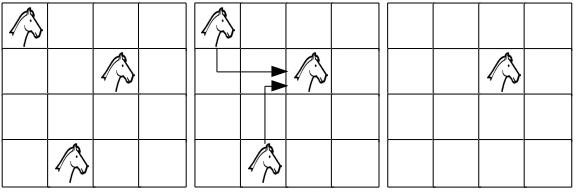
\includegraphics[scale=0.7]{instancia1.jpg}\caption{Problema con $n = 4$, $k = 3$, caballos en (1, 1), (2, 3), (4, 2). Soluci\'on: posición: (2, 3), cantidad de movimientos: 2.}
\vspace{0.2cm}
\centering
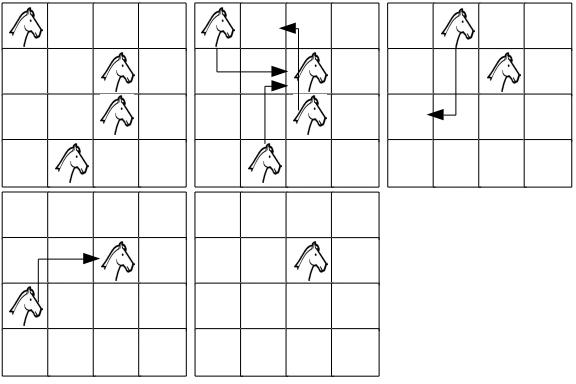
\includegraphics[scale=0.7]{instancia2.jpg}\caption{Problema con $n = 4$, $k = 4$, caballos en (1, 1), (2, 3), (4, 2), (3, 3). Solución: posición (2, 3), cantidad de movimientos: 5.}
\end{figure}

\begin{figure}
\centering
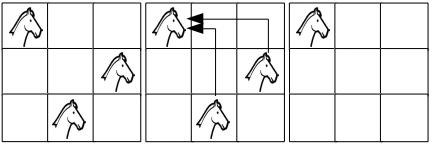
\includegraphics[scale=0.7]{instancia3.jpg}\caption{Problema con $n = 3$, $k = 3$, caballos en (1, 1), (2, 3), (3, 2). Solución: posición (1, 1), cantidad de movimientos: 2.}
\end{figure}

\begin{figure}
\centering
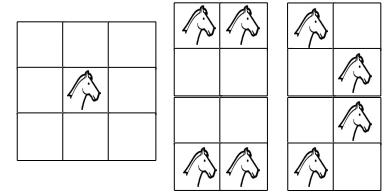
\includegraphics[scale=0.7]{instsinsol.jpg}\caption{El objetivo de esta imagen es analizar las instancias del problema para las cuales lo existe solución. El primer tablero de $n = 3$ podemos observar que tiene un caballo (o más) en la posición (3, 3). Si agregáramos un caballo en \textit{otra} posición del tablero, ya no existiría solución al problema. Esto sucede porque que un caballo en la posición (3, 3) en un tablero de $n = 3$, no puede moverse hacia ninguna otra posición debido a la particularidad de su movimiento, el cual lo obliga a moverse siempre dos posiciones en la misma dirección. Algo similar pasa con los tableros de $n = 2$, donde tampoco se pueden mover los caballos por falta de posiciones en el tablero. Por lo tanto, los cuatro tableros de la derecha representan instancias del problema para las cuales no existe solución.}
\end{figure}

\subsection{Resolución}
Para resolver el problema, vamos a saber de antemano (más adelante explicaremos cómo), cuál es la cantidad mínima de movimientos que debe hacer cada caballo para llegar a una posición partiendo desde su posición inicial (vamos a llamar a esta cantidad $c_{r}^{p}$ para un caballo $r$ y una posición $p$). Sabiendo esto, la dificultad de querer dar una solución (si es que existe) claramente disminuye bastante. La solución, si es que existe, estaría dada por una posicion $t$ del tablero, tal que la suma $S_t = c_{1}^{t} + c_{2}^{t} + ... \ + c_{k}^{t}$ es menor o igual que $S_t'$ para toda posición $t'$ en el tablero y por la suma $S_t$. Es decir, la posición del tablero que minimiza la suma de los movimientos requeridos para llegar a ella partiendo de las posiciones iniciales de cada caballo, junto con la cantidad de movimientos. Basícamente el problema pasaría a ser sacar el mínimo de $n^2$ sumas, lo cual no parece complicado.
\newline La idea es tener los $c_{i}^{p}$ en una matriz $M$ de $k \ $x $ n \ $x $ n$, de manera tal que, si $p = (i, j)$ una posición en el tablero y $r$ un caballo, entonces $M[r][i][j] = c_{r}^{p}$. Entonces después de llenar esa matriz, vamos a tomar para cada posición $(i, j)$ del tablero, la suma sobre todos los caballos (es decir $M[1][i][j] + M[2][i][j] + ... + M[k][i][j]$) y luego tomar el mínimo de todas esas sumas junto con la posición que denota dicho mínimo, como bien dijimos antes.
\newline
\newline Veamos ahora, una idea a grandes rasgos sobre como llenar M para algun caballo $r$, luego daremos el pseudocódigo para que quede mas claro.
\newline Inicialmente $r$ está en una posición $(i, j)$, por lo tanto $M[r][i][j]$ tiene que valer 0 ya que no es necesario hacer ningún movimiento por parte de $r$ para llegar a $(i, j)$ porque es ahí donde empieza estando. Lo que hacemos ahora es fijarnos, a qué posiciones del tablero puede ir $p$ desde $(i, j)$ con un solo movimiento. Estas posiciones van a ser a lo sumo 8 (ver imagen), las guardamos en una lista y ahora repetimos el mismo procedimiento, solo que pensamos a $r$ como si hubiera empezado en cada una de esas 8 posiciones. A la hora de llenar la matriz en cada repetición del proceso, ya no vamos a poner ceros como hicimos con $M[r][i][j]$, si no que vamos a ir incrementando un valor $v$ que será el asignado a la matriz. Dejaremos de iterar cuando, para toda posición $(i', j')$ del tablero, $M[r][i'][j']$ esté definida.

\begin{figure}[h!]
\centering
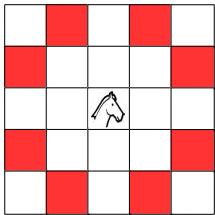
\includegraphics[scale=0.5]{las8.jpg}\caption{El caballo está en $(3, 3)$ y puede ir a las posiciones $(1, 2), (1, 4), (2, 1), (2, 5), (4, 1), (5, 2), (4, 5), (5, 4)$}
\end{figure}

\vspace{0.3cm}
\noindent Hay algunos detalles importantes a tener en cuenta sobre lo explicado arriba. El principal problema es el de los casos repetidos ya que, puede suceder (y de hecho sucede), que al procesar las posiciones a las cuales puedo saltar partiendo desde otra posición, obtenga una posición $p_m$ que ya marqué en la matriz (ver imagen). En este caso decidimos no procesar a $p_m$ y seguir con las otras.

\begin{figure}[h!]
\centering
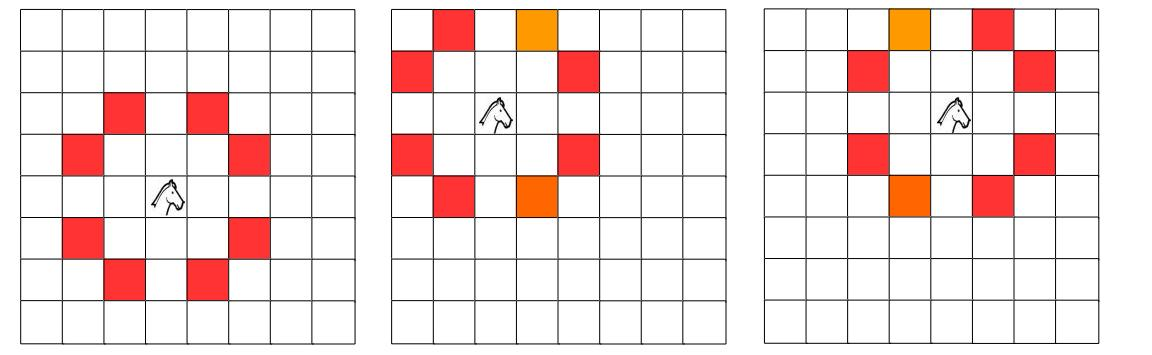
\includegraphics[scale=0.4]{las8repetidas.jpg}\caption{En el primer tablero el caballo está en su posición inicial y mostramos las posiciones posibles a las cuales puede saltar. En el segundo y tercer tablero el caballo ya saltó a una posición y, nuevamente mostramos las posiciónes a las cuales puede moverse desde ahí. Marcamos con naranja las posiciones repetidas. Notemos que, en este caso si procesaramos la posición (1, 4) dos veces, no sería problema ya que de cualquier manera llegamos con dos movimientos. Ahora si procesáramos la posición (1, 4), sí tendríamos problemas, ya que a esa posición se llega con 0 movimientos, por lo tanto si incrementamos $v$ y se lo asignamos a esa posición, estaríamos cometiendo un error. Es por eso que decidimos no procesar posiciones que ya están definidas en la matriz.}
\end{figure}

\noindent A continuación presentamos el pseudocódigo de la función que, dado un caballo $r$ y la matriz $M$, llena $M[r][i'][j']$ para toda $(i', j')$ posición del tablero. Por comodidad, en lugar de trabajar con la matriz $M$ que tiene tres dimensiones, trabajaremos con $M_r$, que representa la matriz de movimientos mínimos para un caballo $r$ particular ($M_r = M[r]$). Dentro del algoritmo, hacemos una llamada a la función PosicionesASaltar, la cual dada una posición y la matriz de movimientos del caballo, nos devuelve una lista con las posiciones válidas a las cuales el caballo puede moverse con un movimiento.
\newline Es importante aclarar que la matriz $M_r$ que LlenarTablero recibe como parámetro, ya tiene asignado 0 en la posición $p$ (el otro parámetro).

\newpage
\begin{algorithmic}[1]
\Procedure{LlenarTablero}{$M_r,p$}
	\State $lista($posición$) \ listaActual \gets$ vacía()
	\State AgregarAtras($listaActual, p$)
	\State $v \gets 0$
	\newline
	\While{$listaActual \neq \ $vacía()}
		\State $lista($posición$) \ listaNueva \gets$ vacía()
		\newline
		\For{$p: \ $posición$ \ in \ listaActual$}
			\State $lista($posición$) \ l \gets$ PosicionesASaltar($p, M_r$)
			\newline
			\For{$paSaltar: \ $posición$ \ in \ l$}
				\State $M_r[paSaltar.i][paSaltar.j] \gets v + 1$
				\State AgregarAtras($listaNueva, paSaltar$)
			\EndFor
			\newline
		\EndFor
		\newline
		\State $listaActual \gets listaNueva$
		\State $v \gets v + 1$
	\EndWhile
	\newline
\EndProcedure
\end{algorithmic}
\vspace{0.5cm}
Debido a que PosicionesASaltar evalúa las 8 posibilidades que mencionamos antes, no vamos a incluir el pseudocódigo. Sin embargo, es importante aclarar que es esta función quien evita que se repitan casos. Al pasarle como parámetro $M_r$, PosicionesASaltar devolverá una lista que contiene a todas las posiciones válidas a las cuales el caballo puede moverse, donde posición válida significa: dentro del tablero, a la cual puede efectivamente moverse con un movimiento y \textit{\textbf{no está marcada ya en la matriz}}.
\newline Una vez que hemos llenado $M_r$ para $r \in [1..k]$, entonces quiere decir que llenamos $M$. Solo queda ver si hay solución y, en el caso de que la haya, devolverla. Como existen casos donde un caballo $r$ directamente \textit{no puede} moverse a alguna posición ($i, j$) del tablero, entonces $M[r][i][j]$ no va a quedar definida. El valor que tomará $M[r][i][j]$ será -1. Es claro que, basta con que exista un solo caballo que no se pueda mover a $(i, j)$ para que $(i, j)$ no forme parte de la solución, por lo tanto, si encontramos ese caballo, descartaremos inmediatamente esa posibilidad.
\newline El pseudocódigo para esta parte del algoritmo es el siguiente:
\vspace{0.4cm}

\begin{algorithmic}[1]
\Procedure{ResolverTablero}{$M$}
	\State $k \gets M.length \ \ \ \ \ \ \ \ \ \ \ \ \ \ //$cantidad de caballos
	\State $n \gets M[0].length \ \ \ \ \ \ \ \ \ \ //$tamaño del tablero
	\State $movsMinimos \gets -1$
	\State $posM$í$nima\ \gets -1$
	\newline
	\For{$i \gets 1$ \textit{\textbf{to} $n$}}
		\For{$j \gets 1$ \textit{\textbf{to} $n$}}
			\State $movs \gets -1$
			\For{$c \gets 1$ \textit{\textbf{to} $k$}}
			\If{$M[c][i][j] = - 1$}
				\State $movs \gets -1$
				\State $\textbf{break}$
			\EndIf
			\State $movs \gets movs + M[c][i][j]$
			\EndFor 
			\If{$(movs < movsMinimos \vee movsMinimos == -1) \wedge movs \neq -1$}
				\State $movsMinimos \gets movs$
				\State $posM$í$nima \gets (i, j)$
			\EndIf
		\EndFor
	\EndFor
	\newline
	\If{$movsMinimos = -1$}
		\State no hay solución
	\Else
		\State la solución es la posición $posM$í$nima$ con la cantidad $movsMinimos$ de movimientos
	\EndIf
	\newline
\EndProcedure
\end{algorithmic}

\vspace{0.5cm}
\noindent Si bien la guarda de la linea 16 puede parecer complicada, lo que hace es fijarse si realmente hay que actualizar o no las variables que representan a una posible solución. Si $movs$ vale -1, entonces claramente debemos descartar $(i, j)$, entonces no cambiamos $movsMinimos$ ni $posMinima$ porque lo mejor que tengo hasta ahora es lo que tenía antes. Si $movs \neq -1$, entonces vamos a cambiar $movsMinimos$ y $posMinima$ solo en el caso de que haya encontrado una posición cuya cantidad de movimientos totales entre todos los caballos sea menor a $movsMinimos$, o $movsMinimos$ valga -1 (en la primera iteración debemos pisar si o si el valor de $movsMinimos$).
\newline Finalmente cuando terminamos de recorrer $M$ y realizar todas las sumas, si $movsMinimos$ nunca cambió, entonces no existe solución al probable, de lo contrario, la solución está en $movsMinimos$ y $posMinima$.
\newline
\newline Entonces el algoritmo completo, lo que hace básicamente es, recibir una lista de posiciones donde cada posición denota un caballo, crear una matriz $M$ de dimensión $k \ $x$\ n \ $x$ \ n$ y, para cada caballo $r$ llenar $M[r]$ llamando a LlenarTablero. Una vez hecho esto, llama a ResolverTablero y termina.

\subsection{Demostración de correctitud}
Comencemos primero por justificar y demostrar porqué $M_r$ va a ser la matriz que contenga, en cada posición $(i, j)$, la cantidad mínima de movimientos necesarios para llegar a $(i, j)$ desde la posición inicial (de ahora en más $(i_0, j_0)$) de $r$.
Pensemos como sería un camino mínimo que realiza un caballo $r$ para llegar a $(i_m, j_m)$ desde $(i_0, j_0)$. Este camino lo podemos ver como una lista $C$ de posiciones, ordenada según a qué posición salta primero $r$. Entonces $C = \ <(i_0, j_0), (i_1, j_1), ... , (i_m, j_m)>$ y $\#C = m + 1$. $C$ claramente no tiene posiciones repetidas, ya que si no, no sería mínimo el camino. Ahora pensemos que valores \textit{\textbf{debería}} tomar $M_r$ para cada posición de la lista: para $(i_0, j_0)$ debería tomar el valor 0 ya que no es necesario efectuar ningún movimiento para llegar a esa posición, debido a que solo asignamos a $M_r[i][j]$ cuando $M_r[i][j] == -1$ y dijimos que cuando efectuamos la llamada a LlenarTablero, $M_r[i_0][j_0] == 0$, esto efectivamente demuestra que $M_r[i_0][j_0]$ tiene el valor correcto; para $(i_1, j_1)$ debería tomar 1 ya que $(i_1, j_1)$ es una de las posiciones a las cuales $r$ se puede mover con un movimiento, desde $(i_0, j_0)$ (si esto no vale entonces $C$ no es un camino válido o tendría una posición repetida, lo cual dijimos que no sucede), y vemos que también se cumple porque, como se trata de una de las 8 posiciones a las cuales $r$ puede moverse desde $(i_0, j_0)$, le es asignado $v + 1$ en la primera iteración del ciclo, donde $v == 0$ por ser justamente la primera iteración; en el caso general entonces, tendremos que $M_r$ en $(i_z, j_z)$ debería tomar $M_r[i_{z-1}][j_{z-1}] + 1$, que representa la cantidad de movimientos necesarios para moverse a la posición anterior, más un movimiento para moverse a la posición actual. Como nuestro algoritmo solo asigna a $M_r[i][j]$ cuando $M_r[i][j] == -1$, entonces nunca pisamos valores que antes asignamos. También, el valor que es asignado por cada iteración, es incrementado, lo cual indica que lo que asignamos a una posición $(i, j)$, siempre va a ser el valor que se le asignará a otra posición $(i', j')$ a la cual $r$ pueda llegar con un solo movimiento desde $(i, j)$. Lo que dijimos hasta ahora, sumado a que siempre consideramos las 8 posiciones a las cuales puede moverse $r$, es argumento suficiente para decir que la igualdad vale.
\newline
\newline Ya vimos que nuestro algoritmo para obtener la matriz de movimientos de un caballo es correcto, resta ver que el ResolverTablero es correcto para concretar la demostración.
\newline Si existe una solución, va a estar dada por una posición del tablero ($posM$í$nima$) y un numero ($movsM$í$nimos$). Queremos ver que $movsM$í$nimos$ cumple ser menor o igual a $S_t$ para toda posición $t$ del tablero y que efectivamente, si sumamos la cantidad de movimientos que le toma a cada caballo llegar a $posM$í$nima$, esa suma nos da $movsM$í$nimos$. 
\newline ResolverTablero pasa por cada posición $(i, j)$ de la matriz (primeros dos fors) y, por cada una de ellas, para cada caballo $c$ (tercer for) si puede moverse o no a $(i, j)$ desde su posición inicial $(i_0, j_0)$. En el caso de que pueda, suma la cantidad de movimientos que le toma hacer eso al caballo, a $movs$ (inicialmente en 0). Si no puede, entonces seguro \textit{\textbf{no formaba parte}} de la solución, por lo tanto sale del for y asigna a $movs$ un valor (-1) que representa que esa posición no debe ser tomada en cuenta. 
\end{document}